\PassOptionsToPackage{hyphens}{url}
\documentclass[compress,aspectratio=169]{beamer}

\usetheme{Reading}

\graphicspath{{../2019-06-isc/}{../2019-06-isc/fig/}{img/}{../logo/}}

\newcommand{\ok}[1]{{#1 (done)}}
\newcommand{\ongoing}[1]{{#1 (ongoing)}}
\newcommand{\started}[1]{{#1 (started)}}
\newcommand{\pending}[1]{{#1 (pending in plan)}}
\newcommand{\hrefb}[2]{\href{#1}{\textcolor{blue}{#2}}}

\subtitle{}
\title{\Large Toward a Globally Acknowledged and Free HPC Certification}
\author{Julian Kunkel (+ HPC Certification Forum)}
\date{2020-05-20}
\authorURL{https://hpc-certification.org}
\authorFooter{Julian M. Kunkel et al.}
\venue{HPCCF Virtual Workshop}
\institute{Department of Computer Science}
\groupLogo{
\includegraphics[width=2.5cm]{hpccf-small}}
\titleLogo{ 
\includegraphics[height=2.5cm]{blur-book-stack-books-590493}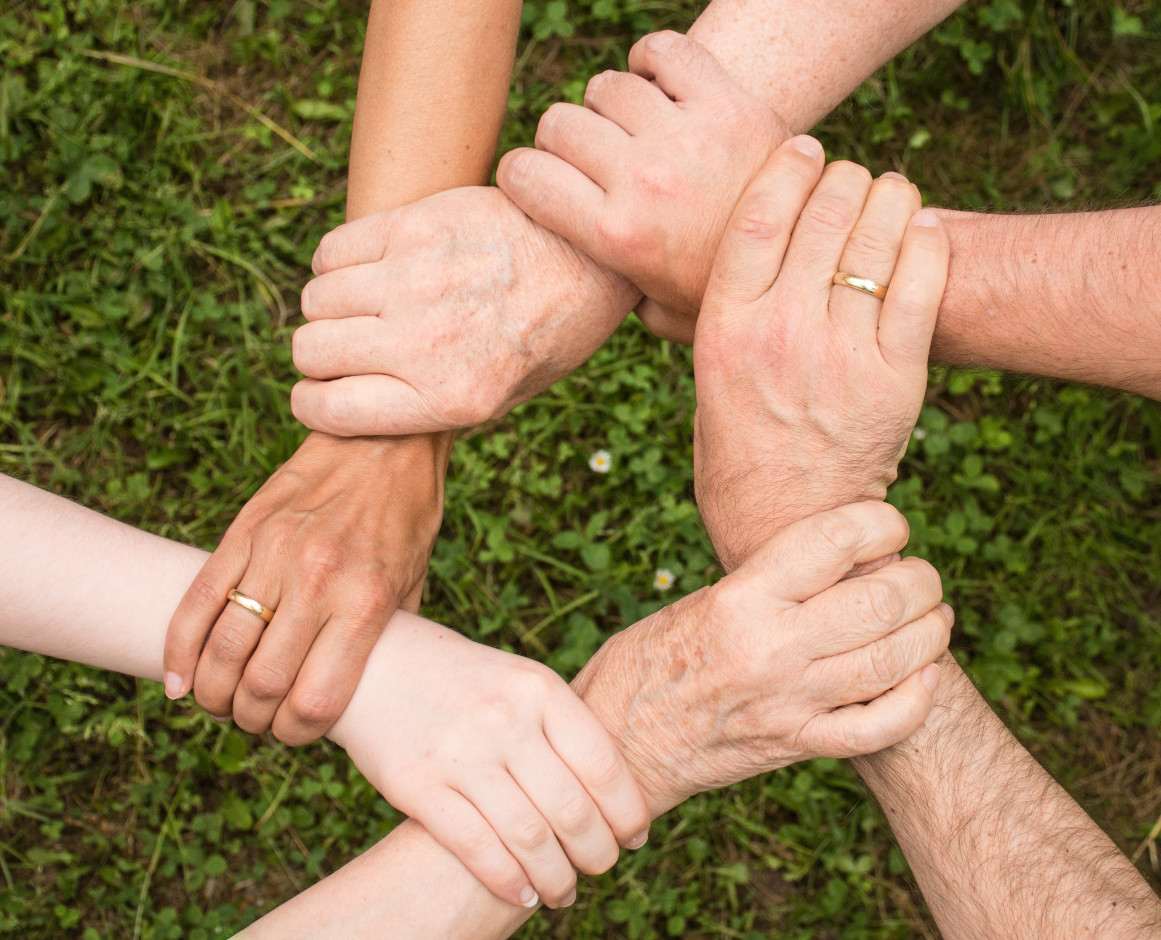
\includegraphics[height=2.5cm]{ground-group-growth-461049}
\includegraphics[height=2.5cm]{accomplishment-ceremony-college-267885}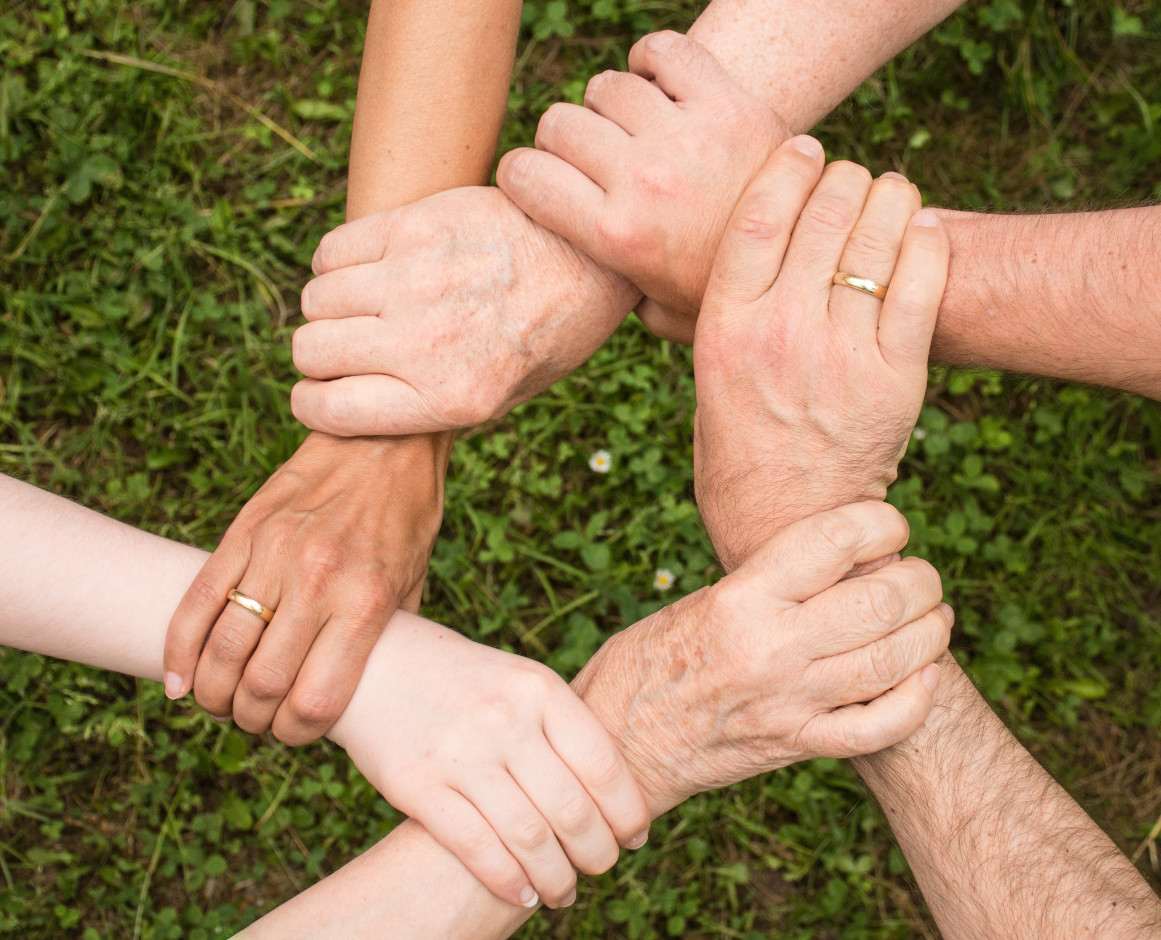
\includegraphics[height=2.5cm]{ground-group-growth-461049}
\includegraphics[height=2.5cm]{blur-book-stack-books-2}}


\begin{document}

\begin{frame}[plain]{}
	\maketitle
\end{frame}

\section{Contributing}

\begin{frame}{High-Level Editing}
  \begin{itemize}
    \item Webpage with Markdown version controlled in Git
      \begin{itemize}
        \item \url{https://www.hpc-certification.org/wiki/skill-tree/b}
        \item GitHub: \url{https://github.com/HPC-certification-forum/skill-tree}
      \end{itemize}
    \item Editing a MindMap, the structure of Skills
      \begin{itemize}
        \item Synchronized with the skill tree in Git
        \item Uses the OpenSource tool Freemind
      \end{itemize}
    \item Discussion on our \href{https://join.slack.com/t/hpc-certification/shared_invite/enQtMzUwNzU3NzM2MTkzLTAzZWM3NDg0N2I2ZmQwOWI5ZGUwNjNlNDgzM2RmOTM3ZWRjNjIxYTc5NzUxYTJhNmRlNmM5YmE1NDY3YzkzYzA}{Slack}
    \item We welcome any contribution via either channel
      \begin{itemize}
        \item Pull requests are also welcome
      \end{itemize}
  \end{itemize}
\end{frame}

\begin{frame}{Webpage}
  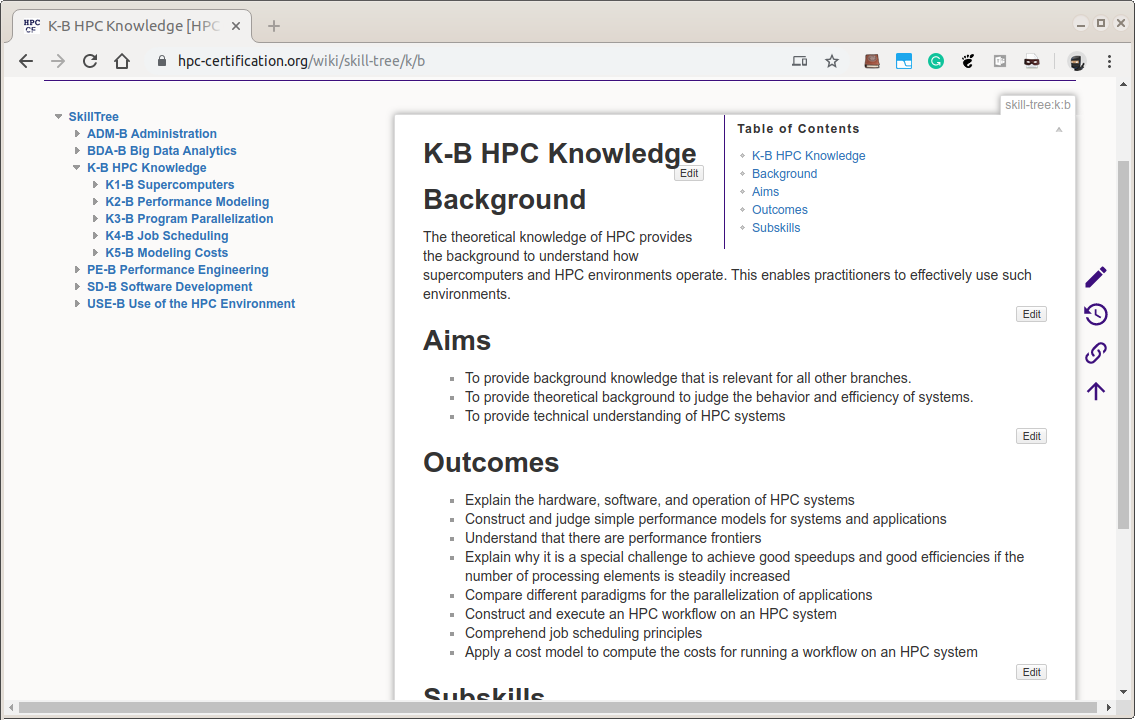
\includegraphics[width=0.8\textwidth]{www}
\end{frame}



\section{Certification Process}
\sectionIntroHidden

\begin{frame}{Certification: Assessment Prototype}
		\begin{itemize}
			\item[\color{readingRed}{1.}] User takes multiple-choice test online (any time!)
			\begin{itemize}
				\item A combination of JavaScript and a web service
				\item System selects number of questions randomly from a pool
					\begin{itemize}
						\item The questions are managed with rigorous license agreement
					\end{itemize}
				\item System draws 4-5 responses from 10 possible responses (some randomized)
			\end{itemize}
			\item[\color{readingRed}{2.}] Choices are submitted to the web server
			\item[\color{readingRed}{3.}] \textit{Manual approval} of the result
			\item[\color{readingRed}{4.}] Automatic creation of certificate and returned by email
			\begin{itemize}
							\item Permanent computer-verifiable proof that skill is created
							\begin{itemize}
								\item Return a text version with GPG signature
								\item Return a link that can be verified on hpc-certification.org
							\end{itemize}
			\end{itemize}
			\item Privacy: minimize information stored on servers, keep some for statistics
			\item Includes some measure to prevent cheating and brute forcing (e.g., delay)
		\end{itemize}
\end{frame}

\begin{frame}[fragile]{Certification: Certificate}
\begin{columns}
	\column{0.6\textwidth}
	\begin{block}{Text representation}

		\scriptsize
		\begin{verbatim}
-----BEGIN PGP SIGNED MESSAGE-----
Hash: SHA512
HPC Certification Forum Certificate
This text confirms that "Jane Doe" has
successfully obtained the certificate
"HPC driving license" (id: 1) at 02/2019.
Verification URL: https://hpc-certification.org/[...]
-----BEGIN PGP SIGNATURE-----
[...]
-----END PGP SIGNATURE-----
		\end{verbatim}
	\end{block}

\column{0.4\textwidth}
	\begin{block}{Certificate}
		\medskip
		
\includegraphics[width=\textwidth]{jane-doe}
	\end{block}
\end{columns}
\end{frame}



\section{Conclusions}
\sectionIntroHidden


\begin{frame}{Summary}

	\begin{block}{HPC Certification Program}
		\begin{itemize}
			\item xx
		\end{itemize}
	\end{block}
\end{frame}




\end{document}
